CausClass gồm ba giai đoạn vận hành nối tiếp. Giai đoạn 1 phát hiện, theo dõi và gom hành vi lớp học từ video thành chuỗi thời gian đa biến. Giai đoạn 2 tìm kiếm đồ thị liên kết thời gian trên chuỗi đó bằng AERCA, bộ sinh đề xuất LLM và beam search. Giai đoạn 3 chuyển tóm tắt chuỗi thời gian và các cạnh đồ thị đã kiểm chứng thành báo cáo quan sát theo nguyên tắc evidence-first. Báo cáo bị ràng buộc có chủ đích: phải nêu dữ kiện phát hiện trước, diễn giải cạnh đồ thị một cách thận trọng và khuyến nghị con người kiểm tra lại video trước mọi hành động trong lớp học.

\begin{figure}[htbp]
  \centering
  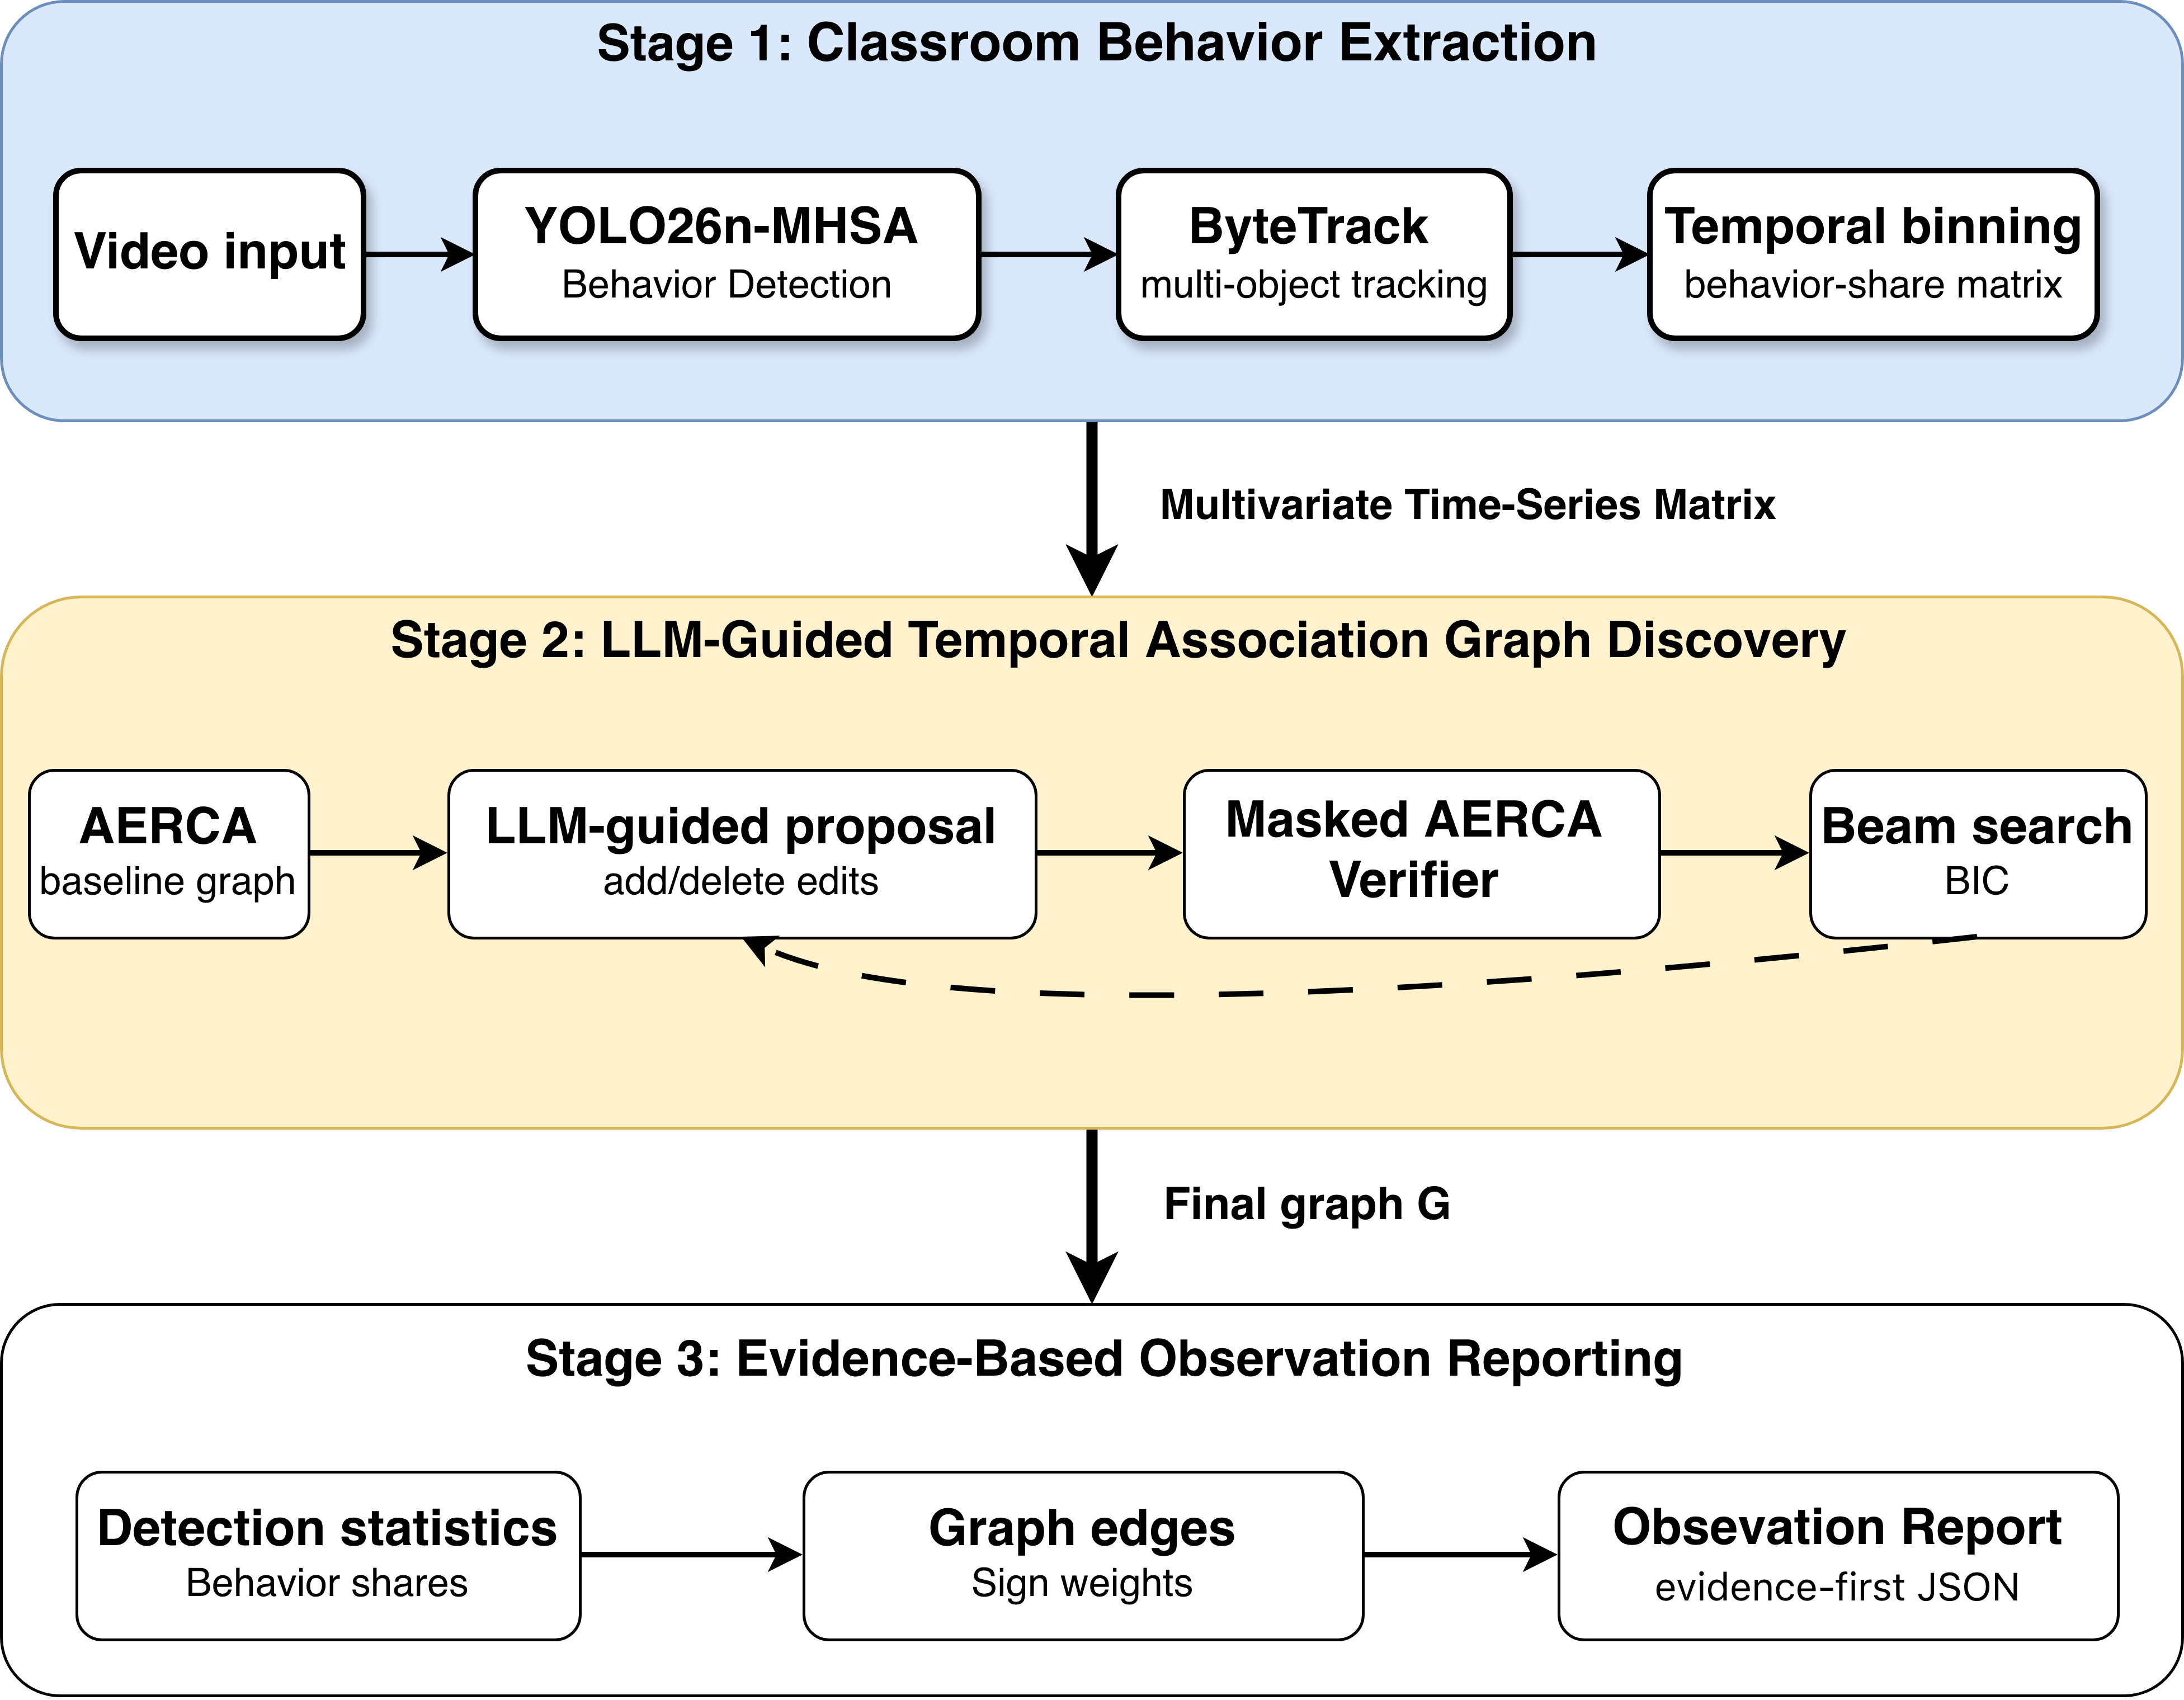
\includegraphics[width=0.95\textwidth]{figures/overall.png}
  \caption{Tổng quan pipeline CausClass. Hệ thống được chia thành ba giai đoạn: trích xuất chuỗi thời gian hành vi từ video, khám phá liên kết thời gian và sinh báo cáo quan sát dựa trên bằng chứng.}
  \label{fig:causclass-overview}
\end{figure}

Hình~\ref{fig:causclass-overview} tóm tắt luồng dữ liệu của toàn hệ thống. Sự tách biệt giữa các giai đoạn là một cơ chế an toàn quan trọng. Phát hiện và theo dõi chỉ tạo bằng chứng quan sát; tìm kiếm đồ thị chỉ tóm tắt cấu trúc dự báo theo thời gian; sinh báo cáo chỉ chuyển các bằng chứng đã có thành văn bản dễ đọc. Không giai đoạn nào được phép tự nâng cấp liên kết quan sát thành kết luận nhân quả chắc chắn hoặc kết luận sư phạm cuối cùng.

Luồng dữ liệu chính có thể viết dưới dạng
\begin{equation}
\label{eq:causclass-pipeline}
    V \rightarrow \mathcal{E} \rightarrow X \rightarrow G^\star \rightarrow R,
\end{equation}
trong đó \(V\) là video đầu vào, \(\mathcal{E}\) là tập sự kiện hành vi sau phát hiện và theo dõi, \(X\in\mathbb{R}^{T\times K}\) là chuỗi thời gian hành vi gồm \(T\) time bin và \(K\) biến hành vi, \(G^\star\) là đồ thị liên kết thời gian cuối cùng và \(R\) là báo cáo quan sát. Mỗi mũi tên là một phép biến đổi có artifact trung gian: khung debug, file sự kiện vi mô, CSV chuỗi thời gian, danh sách cạnh, ma trận kề và báo cáo. Thiết kế này giúp truy vết lỗi: nếu báo cáo có nhận xét bất thường, người dùng có thể quay lại cạnh đồ thị, chuỗi thời gian, sự kiện phát hiện hoặc khung hình gốc.

Trong giai đoạn perception và temporal abstraction, detector YOLO26n-MHSA tạo các hộp phát hiện hành vi theo từng khung hình. ByteTrack liên kết các hộp này thành track để giảm đứt đoạn ngắn và tạo sự kiện có thời gian bắt đầu--kết thúc; các sự kiện sau đó được gom theo time bin thành tỉ lệ hành vi. Trong giai đoạn temporal discovery, AERCA cung cấp đồ thị ban đầu và tín hiệu hệ số. LLM không trực tiếp quyết định đồ thị; nó chỉ đề xuất chỉnh sửa, còn masked AERCA và điểm số BIC-style đánh giá ứng viên. Trong giai đoạn reporting, đồ thị đã kiểm chứng và tóm tắt chuỗi thời gian được render thành báo cáo có ràng buộc, không cho phép đổi chiều cạnh hoặc phát minh quan hệ mới.

Nguyên tắc thiết kế xuyên suốt là phân tách vai trò giữa quan sát, kiểm chứng và diễn giải. Detector trả lời câu hỏi ``hành vi nào được nhìn thấy''. Mô hình thời gian trả lời câu hỏi ``tín hiệu nào có ích cho dự báo tín hiệu nào''. Báo cáo trả lời câu hỏi ``người dùng nên kiểm tra điều gì trong video''. Nhờ phân tách này, CausClass phù hợp với dữ liệu lớp học quan sát thụ động: hệ thống hỗ trợ phân tích và đặt giả thuyết, nhưng không thay thế chuyên gia giáo dục trong việc xác định ý nghĩa sư phạm.